\section{Approach}
\label{sec:approach}

This section presents our methodology for systematically generating adversarial scenarios to evaluate autonomous driving systems. Our approach has the following workflow: Sec.~\ref{sec:typology_selection} selects and justifies ten target pre-crash typologies from the NHTSA classification, grouped into three kinematic categories. Sec.~\ref{sec:threshold_selection} then establishes a two-tier threat metric framework, with threshold values derived from Euro~NCAP protocols, that provides the quantitative criteria for identifying seed scenarios and evaluating generated candidates. Finally, Sec.~\ref{sec:generation} details the adversarial generation pipeline itself, which transforms real-world near-miss events into analytically more critical test cases through parameterized perturbation, open-loop analytical optimisation, and diversity-driven selection.
\subsection{Target Pre-Crash Typology Selection}\label{sec:typology_selection}
\begin{figure}
    \centering
    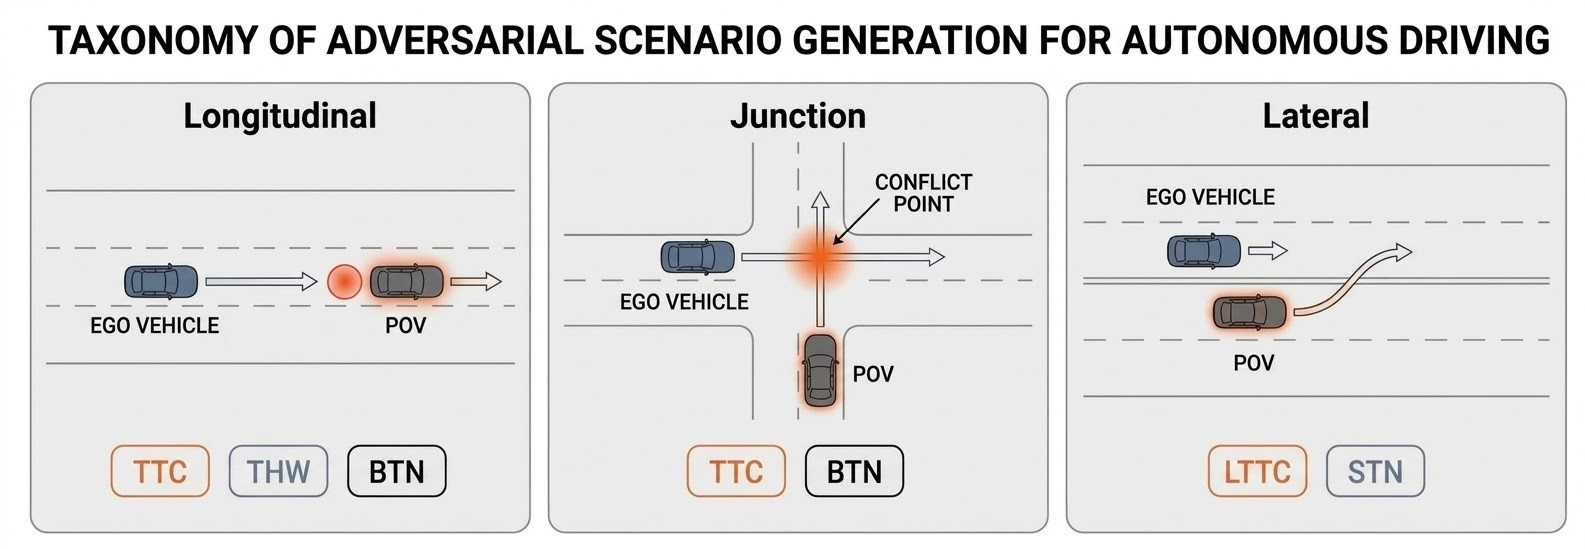
\includegraphics[width=\linewidth]{imgs/scenario_taxonomy.png}
    \caption{Visual taxonomy of the three kinematic categories, their spatial configurations, associated threat metrics, and adversarial generation strategies.}

    \label{fig:scenario_taxonomy}
\end{figure}
\begin{table*}[t]
  \caption{Categorization of NHTSA Pre-Crash Scenarios and Target Threat Metrics}
  \label{tab:kinematic_categories}
  \renewcommand{\arraystretch}{1.0} 
  \begin{tabularx}{\textwidth}{@{} 
      >{\hsize=0.25\hsize\raggedright\arraybackslash}X 
      >{\hsize=0.50\hsize\raggedright\arraybackslash}X 
      >{\hsize=0.25\hsize\raggedright\arraybackslash}X 
      @{}}
    \toprule
    \textbf{Kinematic Category} & \textbf{Included Typologies (NHTSA)} & \textbf{Target Metrics} \\
    \midrule
    
    \rowcolor{blue!5}
    \textbf{Longitudinal} & 
    (1) Lead Vehicle Stopped \newline 
    (2) Lead Vehicle Decelerating \newline 
    (3) Lead Veh. Moving at Lower Speed & 
    TTC, THW, BTN \\
    
    \rowcolor{green!5}
    \textbf{Junction} & 
    (4) Veh. Turning at Non-Signalized \newline 
    (5) Straight Crossing Non-Signalized \newline 
    (6) LTAP/OD at Signalized \newline 
    (7) LTAP/OD at Non-Signalized & 
    TTC, BTN \\
    
    \rowcolor{orange!5}
    \textbf{Lateral} & 
    (8) Veh. Changing Lanes (Same Dir.) \newline 
    (9) Veh. Turning (Same Dir.) \newline
    (10) Vehicle Drifting (Same Dir.) & 
    LTTC, STN \\
    
    \bottomrule
  \end{tabularx}
\end{table*}

% \begin{table*}[t]
%   \caption{Categorization of NHTSA Pre-Crash Scenarios and Target Threat Metrics}
%   \label{tab:kinematic_categories}
%   \renewcommand{\arraystretch}{1.2} 
%   \begin{tabularx}{\textwidth}{@{} 
%       >{\hsize=0.25\hsize\raggedright\arraybackslash}X 
%       >{\hsize=0.50\hsize\raggedright\arraybackslash}X 
%       >{\hsize=0.25\hsize\raggedright\arraybackslash}X 
%       @{}}
%     \toprule
%     \textbf{Kinematic Category} & \textbf{Included Typologies (NHTSA)} & \textbf{Target Metrics} \\
%     \midrule
    
%     \rowcolor{blue!5}
%     \textbf{Longitudinal} & 
%     (1) Lead Vehicle Stopped \newline 
%     (2) Lead Vehicle Decelerating \newline 
%     (3) Lead Veh. Moving at Lower Speed & 
%     TTC, THW, BTN \\
%     \addlinespace
    
%     \rowcolor{green!5}
%     \textbf{Junction} & 
%     (4) Veh. Turning at Non-Signalized \newline 
%     (5) Straight Crossing Non-Signalized \newline 
%     (6) LTAP/OD at Signalized \newline 
%     (7) LTAP/OD at Non-Signalized & 
%     TTC, BTN \\
%     \addlinespace
    
%     \rowcolor{orange!5}
%     \textbf{Lateral} & 
%     (8) Veh. Changing Lanes (Same Dir.) \newline 
%     (9) Veh. Turning (Same Dir.) \newline
%     (10) Vehicle Drifting (Same Dir.) & 
%     LTTC, STN \\
    
%     \bottomrule
%   \end{tabularx}
% \end{table*}
We select ten pre-crash typologies from the NHTSA Pre-Crash Scenario Typology for Crash Avoidance Research~\cite{noauthor_pre-crash_nodate}, drawing from two-vehicle crash scenarios ranked by frequency of occurrence. The nine highest-frequency typologies are retained directly: (1)~Lead Vehicle Stopped (20.46\%), (2)~Vehicle(s) Turning at Non-Signalized Junctions (10.83\%), (3)~Lead Vehicle Decelerating (8.96\%), (4)~Vehicle(s) Changing Lanes -- Same Direction (7.62\%), (5)~Straight Crossing Paths at Non-Signalized Junctions (6.52\%), (7)~Vehicle(s) Turning -- Same Direction (5.68\%), (8)~LTAP/OD at Signalized Junctions (5.29\%), (9)~Lead Vehicle Moving at Lower Constant Speed (4.82\%), and (10)~LTAP/OD at Non-Signalized Junctions (4.68\%). Together, these nine scenarios account for approximately 71\% of all two-vehicle light-vehicle crashes. The sixth-ranked typology, Running Red Light (6.02\%), is excluded because it constitutes an explicit traffic rule violation rather than a legitimate driving behaviour which falls outside this scope, and would be more appropriately addressed through traffic signal compliance testing rather than kinematic perturbation of the POV. In its place, we include the thirteenth-ranked typology, Vehicle(s) Drifting -- Same Direction (2.35\%), which complements the lateral kinematic category by introducing a gradual lane encroachment maneuver distinct from the abrupt lane changes captured by typology~4. This substitution ensures comprehensive coverage of lateral conflict dynamics while maintaining a physically parameterizable search space across all ten selected typologies. The ten typologies are grouped into three kinematic categories --- longitudinal, junction, and lateral --- based on the dominant conflict direction, as summarised in Table~\ref{tab:kinematic_categories} and illustrated in Fig.~\ref{fig:scenario_taxonomy}. Each category is associated with a distinct set of threat metrics that govern the objective function for scenario generation.
\begin{figure*}[t]
    \centering
    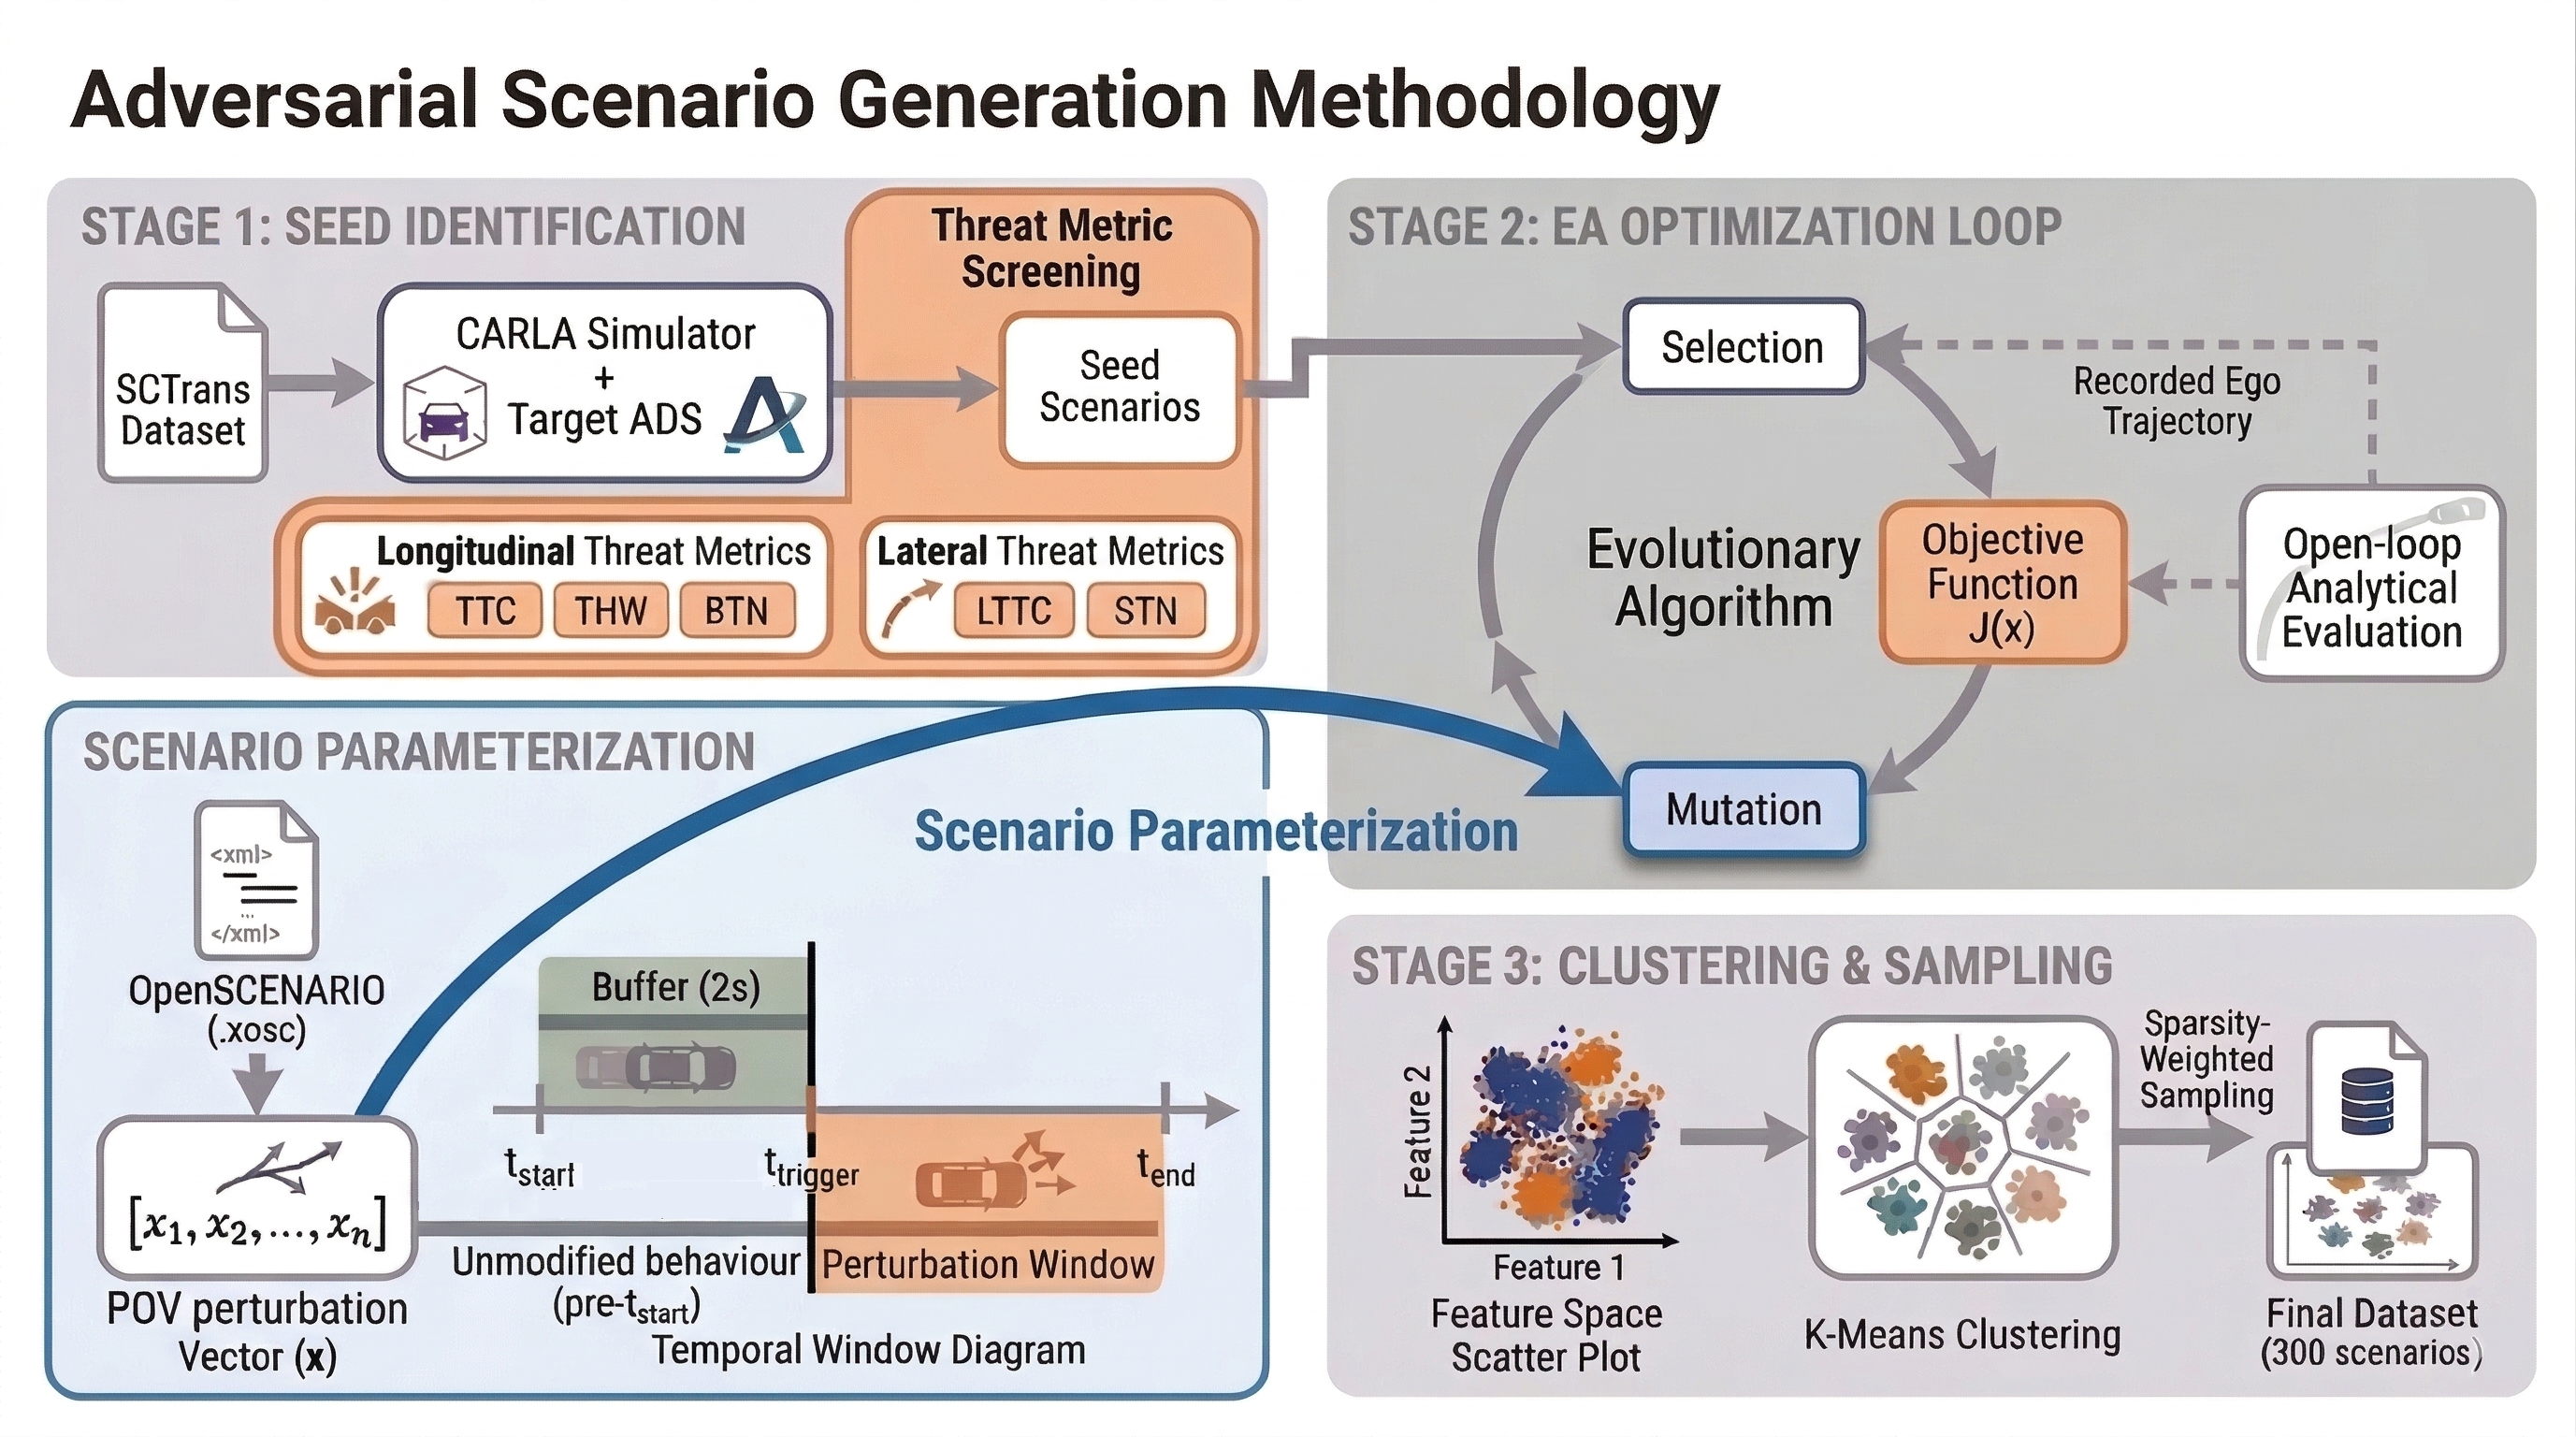
\includegraphics[width=0.8\textwidth]{imgs/generation_workflow.jpg}
    \caption{Overview of the adversarial scenario generation pipeline: seed identification via threat metric screening, scenario parameterization with temporal windowing, evolutionary algorithm optimization using open-loop analytical evaluation, and diversity-driven clustering and sampling.}

    \label{fig:generation_workflow}
\end{figure*}

\subsection{Threat Metrics and Threshold Selection}
\label{sec:threshold_selection}
To identify safety-critical scenarios from the broader dataset, we require a principled method for quantifying collision risk during baseline simulations. We employ five kinematic threat metrics grouped by the dominant conflict direction. The metrics and their associated thresholds provide the quantitative foundation for both seed scenario identification and adversarial scenario evaluation.
\subsubsection{Threat Metric Definitions}
\label{sec:threat_metrics}

For longitudinal and junction conflicts, we define three metrics that capture temporal proximity and braking demand. Time-to-Collision (TTC) and Time Headway (THW) measure the temporal margin available to the ego vehicle, while the Brake Threat Number (BTN) quantifies the required deceleration relative to the vehicle's physical braking limit:
\begin{equation}
    \text{TTC} = \frac{x_{rel}}{v_{x, rel}}, \quad \text{THW} = \frac{x_{rel}}{v_{ego}}, \quad \text{BTN} = \frac{a_{x, req}}{a_{x, max}}
\end{equation}
where $x_{rel}$ and $v_{x, rel}$ are the relative longitudinal distance and velocity, $v_{ego}$ is the ego vehicle's speed, $a_{x, req}$ is the required deceleration to avoid collision, and $a_{x, max}$ is the vehicle's maximum physical braking limit. Lower TTC and THW values indicate greater temporal urgency, while higher BTN values indicate greater braking severity. To prevent mathematical instability when $v_{x, rel}$ approaches zero, the upper bounds of TTC and THW are capped at their corresponding critical thresholds as specified in Table~\ref{tab:thresholds}.

For lateral conflicts such as lane changing and drifting, $v_{x, rel}$ approaches zero, rendering TTC mathematically unstable. We therefore substitute the longitudinal metrics with Lateral Time-to-Collision (LTTC) and Steering Threat Number (STN):
\begin{equation}
    \text{LTTC} = \frac{y_{rel}}{v_{y, rel}}, \quad \text{STN} = \frac{a_{y, req}}{a_{y, max}}
\end{equation}
where $y_{rel}$ and $v_{y, rel}$ are the relative lateral distance and velocity, $a_{y, req}$ is the required lateral evasion acceleration, and $a_{y, max}$ is the maximum lateral acceleration capacity governed by road friction limits. The assignment of metrics to kinematic categories follows Table~\ref{tab:kinematic_categories}.

\subsubsection{Threshold Selection}
\label{sec:thresholds}
Each metric is assigned a two-tier threshold structure. The \textit{critical} tier identifies the onset of a safety-relevant interaction and is used to filter baseline simulations for near-miss events that serve as seed scenarios for adversarial generation. The \textit{emergency} tier defines the boundary of an unavoidable conflict and serves as the threat threshold for the optimisation process: candidate scenarios must drive at least one metric beyond its emergency threshold to be retained. The threshold values, summarised in Table~\ref{tab:thresholds}, are derived from the Euro~NCAP Assisted Driving Highway \& Interurban Test and Assessment Protocol v2.2~\cite{noauthor_euro_nodate}.

\begin{table}[htbp]
\centering
\caption{Threat metric thresholds derived from the Euro~NCAP Assisted Driving Highway \& Interurban Test and Assessment Protocol v2.2~\cite{noauthor_euro_nodate}.}
\label{tab:thresholds}
\renewcommand{\arraystretch}{1.0}
\begin{tabular}{@{}llcl@{}}
\toprule
\textbf{Metric} & \textbf{Level} & \textbf{Value} & \textbf{Derivation Basis} \\
\midrule
\multirow{2}{*}{TTC}
  & Critical  & 3.0  & ACC abort criterion (\S3.3.1.1)          \\
  & Emergency & 1.5  & FCW issuance threshold (\S4.3.1)         \\
\multirow{2}{*}{THW}
  & Critical  & 2.0  & ISO~15622 upper bound   \\
  & Emergency & 1.0  & ACC minimum gap (\S3.3.1.1)   \\
\multirow{2}{*}{BTN}
  & Critical  & 0.52 & CCRs (\S3.3.1) \\
  & Emergency & 0.80 & ACC-to-AEB transition (\S4.3.1)   \\
\multirow{2}{*}{LTTC}
  & Critical  & 1.5  & Cut-in TTC (\S3.3.1.3)   \\
  & Emergency & 0.5  & C2MC cut-in TTC (\S3.3.2.5) \\
\multirow{2}{*}{STN}
  & Critical  & 0.40 & Lane Support System (\S4.3.5) \\
  & Emergency & 0.64 & S-Bend (\S3.4.1) \\
\bottomrule
\end{tabular}
\end{table}

% \begin{table}[htbp]
% \centering
% \caption{Threat metric thresholds for autonomous driving scenario evaluation, derived from the Euro~NCAP Assisted Driving Highway \& Interurban Test and Assessment Protocol v2.2~\cite{noauthor_euro_nodate}.}
% \label{tab:thresholds}
% \renewcommand{\arraystretch}{1.3}
% \begin{tabular}{@{}llcl@{}}
% \toprule
% \textbf{Metric} & \textbf{Level} & \textbf{Value} & \textbf{Derivation Basis} \\
% \midrule
% \multirow{2}{*}{TTC}
%   & Critical  & 3.0  & ACC abort criterion (\S3.3.1.1)          \\
%   & Emergency & 1.5  & FCW issuance threshold (\S4.3.1)         \\
% \midrule
% \multirow{2}{*}{THW}
%   & Critical  & 2.0  & ISO~15622 upper bound   \\
%   & Emergency & 1.0  & ACC minimum gap (\S3.3.1.1)   \\
% \midrule
% \multirow{2}{*}{BTN}
%   & Critical  & 0.52 & CCRs (\S3.3.1) \\
%   & Emergency & 0.80 & ACC-to-AEB transition (\S4.3.1)   \\
% \midrule
% \multirow{2}{*}{LTTC}
%   & Critical  & 1.5  & Cut-in TTC (\S3.3.1.3)   \\
%   & Emergency & 0.5  & C2MC cut-in TTC (\S3.3.2.5) \\
% \midrule
% \multirow{2}{*}{STN}
%   & Critical  & 0.40 & Lane Support System (\S4.3.5) \\
%   & Emergency & 0.64 & S-Bend (\S3.4.1) \\
% \bottomrule
% \end{tabular}
% \end{table}

Of the ten threshold values, four (TTC critical and emergency, LTTC critical and emergency) are directly mapped from explicitly stated protocol parameters --- test abort criteria, warning issuance deadlines, and prescribed TTC values at lane-change completion. The remaining six are derived from the protocol's test configurations through established physical relationships: THW values from the closest following distance requirement, BTN values from the most demanding ACC scenario (CCRs) and the ACC-to-AEB transition boundary, and STN values from the LKA departure threshold and the S-Bend lateral acceleration demand.
% \subsubsection{Threshold Selection}
% \label{sec:thresholds}

% Each metric is assigned a two-tier threshold structure. The \textit{critical} tier identifies the onset of a safety-relevant interaction and is used to filter baseline simulations for near-miss events that serve as seed scenarios for adversarial generation. The \textit{emergency} tier defines the boundary of an unavoidable conflict and serves as the threat threshold for the optimisation process: candidate scenarios must drive at least one metric beyond its emergency threshold to be retained. The threshold values, summarised in Table~\ref{tab:thresholds}, are derived from the Euro~NCAP Assisted Driving Highway \& Interurban Test and Assessment Protocol v2.2~\cite{noauthor_euro_nodate}.

% \begin{table}[htbp]
% \centering
% \caption{Threat metric thresholds for autonomous driving scenario evaluation, derived from the Euro~NCAP Assisted Driving Highway \& Interurban Test and Assessment Protocol v2.2~\cite{noauthor_euro_nodate}.}
% \label{tab:thresholds}
% \renewcommand{\arraystretch}{1.3}
% \begin{tabular}{@{}llcl@{}}
% \toprule
% \textbf{Metric} & \textbf{Level} & \textbf{Value} & \textbf{Derivation Basis} \\
% \midrule
% \multirow{2}{*}{TTC}
%   & Critical  & 3.0  & ACC abort criterion (\S3.3.1.1)          \\
%   & Emergency & 1.5  & FCW issuance threshold (\S4.3.1)         \\
% \midrule
% \multirow{2}{*}{THW}
%   & Critical  & 2.0  & ISO~15622 upper bound   \\
%   & Emergency & 1.0  & ACC minimum gap (\S3.3.1.1)   \\
% \midrule
% \multirow{2}{*}{BTN}
%   & Critical  & 0.52 & CCRs (\S3.3.1) \\
%   & Emergency & 0.80 & ACC-to-AEB transition (\S4.3.1)   \\
% \midrule
% \multirow{2}{*}{LTTC}
%   & Critical  & 1.5  & Cut-in TTC (\S3.3.1.3)   \\
%   & Emergency & 0.5  & C2MC cut-in TTC (\S3.3.2.5) \\
% \midrule
% \multirow{2}{*}{STN}
%   & Critical  & 0.40 & Lane Support System (\S4.3.5) \\
%   & Emergency & 0.64 & S-Bend (\S3.4.1) \\
% \bottomrule
% \end{tabular}
% \end{table}

% Of the ten threshold values, four are \textit{directly mapped} from explicitly stated protocol parameters. The TTC critical threshold of 3.0\,s corresponds to the test abort criterion specified in (\S3.3.1.1), whereby a trial is terminated if the ACC system has not initiated braking by this point. The TTC emergency threshold of 1.5\,s is the forward collision warning (FCW) issuance deadline in (\S4.3.1), below which partial credit is awarded only if a warning has been provided. The LTTC thresholds of 1.5\,s and 0.5\,s correspond directly to the prescribed TTC values at lane-change completion for the car-to-car cut-in test (\S3.3.1.3) and the car-to-motorcyclist cut-in test (\S3.3.2.5), respectively.

% The remaining six thresholds are \textit{derived} from the protocol's test configurations through established physical relationships. The THW values of 2.0\,s (critical) and 1.0\,s (emergency) are inferred from the protocol's requirement to test at the ``closest following distance'' (\S3.3.1.1). The BTN critical value of 0.52 is computed from the most demanding ACC scenario---CCRs. The BTN emergency value of 0.80 marks the transition into the AEB operating regime, where deceleration demands exceed the ACC comfort boundary. The STN critical value of 0.40 is mapped from the protocol's LKA departure threshold (\S4.3.5), which awards points only when lane departure is limited to 0.4\,m. The STN emergency value of 0.64 is derived from the lateral acceleration demand of the S-Bend second turn.

\subsection{Adversarial Scenario Generation -- Regular Setting}\label{sec:generation}
Building on the ten target typologies and their associated threat metrics defined in Sec.~\ref{sec:typology_selection} and~\ref{sec:threshold_selection}, this section presents the adversarial scenario generation pipeline. The core objective is to transform near-miss traffic events into more critical, collision-likely test cases without violating physical plausibility. An overview of the complete pipeline is illustrated in Fig.~\ref{fig:generation_workflow}. The pipeline begins with an empirical screening phase, simulating 854 real-world traffic events from the SCTrans dataset in the CARLA simulator to identify vulnerable ``seed'' scenarios which trigger the predefined threat metrics corresponding to each typology. We frame the adversarial generation as a constrained optimization problem. By parameterizing the dynamic behavior of the Principal Other Vehicle (POV) within the OpenSCENARIO framework and constraining these bounds to Euro NCAP regulatory standards, we maintain strict kinematic realism. An evolutionary algorithm (EA) iteratively perturbs these variables using open-loop analytical evaluation against recorded ego-vehicle trajectories, guided by the typology-specific objective function. A key contribution of this methodology is the open-loop analytical optimization with temporally scoped perturbations (Sec.~\ref{sec:seed}): by restricting modifications to the threat-metric-triggered window and evaluating against recorded baseline trajectories, we achieve efficient search-space exploration while maintaining the physical validity of each generated scenario. Finally, feature-space clustering with sparsity-weighted sampling distills the results into 300 highly diverse, representative failure modes across all ten typologies.

\subsubsection{Seed Scenario Identification and Parameterization}\label{sec:seed}
% \subsection{Adversarial Behaviours Supported}
% - include a table on the different types of adversarial behaviour


The adversarial generation pipeline begins with the empirical identification of high-risk baseline events. We execute 854 original, unperturbed scenarios from the SCTrans dataset within the CARLA simulator, utilizing Apollo as the target ego vehicle. During these baseline simulations, we continuously monitor the kinematic interactions between the ego vehicle and the surrounding traffic. Scenarios that breach safe operational thresholds and trigger our target threat metrics (TTC, THW, and BTN for longitudinal conflicts; LTTC and STN for lateral conflicts) are classified as near-misses and extracted as foundational ``seed'' scenarios. The threshold values defining these near-miss boundaries are established in Sec~\ref{sec:threshold_selection}.

Once these vulnerable seeds are identified, their existing OpenSCENARIO (\texttt{.xosc}) definitions are restructured to decouple the static environment from the parameterized adversarial agent. The map topology, defined in the corresponding \texttt{.xodr} files, remains unchanged. Static environmental constraints and background non-POV traffic within the \texttt{.xosc} files are preserved, constrained to their recorded trajectories, to maintain the baseline realism of the SCTrans data. Conversely, the dynamic state of the Principal Other Vehicle (POV)---the primary adversarial agent---is parameterized to form a continuous search space. Crucially, we do not modify the entire scenario timeline. For each seed, we identify the temporal window during which the threat metrics are actively triggered, and restrict perturbations exclusively to this window plus a 2-second preceding buffer. This buffer allows the POV to transition smoothly from its unmodified baseline behavior to the perturbed, higher-risk state. All behavior prior to this window remains identical to the original scenario, ensuring that the ego vehicle's recorded trajectory up to the onset of the perturbation window is valid and unaffected.

We define a perturbation vector $\mathbf{x}$ for each seed, encompassing variables such as the POV's initial velocity ($v_{POV}$) and acceleration profiles ($a_{POV}$). We utilize OpenSCENARIO triggers, specifically the \texttt{RelativeDistanceCondition}, \texttt{RelativeSpeedCondition}, to define the exact spatial and velocity thresholds at which the POV executes risky behaviors, such as a sudden brake within a critical time window when the ego vehicle is trailing, or an aggressive lane change. By directly modifying these parameters within the \texttt{.xosc} XML structure, we create a controllable testbed ready for heuristic optimization.

\subsubsection{Defining the Objective Function}\label{sec:objective}
To guide the search algorithm toward a collision state, we formulate a fitness function $J(\mathbf{x})$ that quantitatively evaluates the danger of each candidate trajectory. The function is designed such that lower values of $J(\mathbf{x})$ indicate higher collision risk, and the evolutionary algorithm seeks to minimize it. The unified objective function is formulated as:
\begin{equation}
    J(\mathbf{x}) = \sum_{i} \mathcal{T}_{i}(\mathbf{x}) - \sum_{j} \mathcal{R}_{j}(\mathbf{x})
\end{equation}
where $\mathcal{T}_{i}(\mathbf{x})$ denotes the time-based proximity metrics (TTC/THW for longitudinal conflicts, or LTTC for lateral conflicts) and $\mathcal{R}_{j}(\mathbf{x})$ denotes the threat number metrics (BTN for longitudinal conflicts, or STN for lateral conflicts), as defined in Sec.~\ref{sec:threat_metrics}. The time-based metrics decrease as collision risk increases, while the threat numbers increase with risk; subtracting the latter ensures that all terms contribute consistently toward a lower $J(\mathbf{x})$ for higher-risk scenarios. All metrics are weighted equally, as they capture complementary aspects of collision risk: temporal margins and the required evasive effort. Minimizing $J(\mathbf{x})$ therefore simultaneously drives the scenario toward shorter time margins and greater difficulty for the ego vehicle to avoid collision.

\subsubsection{Optimization and Search Algorithm}\label{sec:optimization}
We model the generation pipeline as a constrained optimization problem, utilizing an Evolutionary Algorithm (EA) to iteratively evolve the perturbation vector $\mathbf{x}$ toward a critical collision boundary. To ensure that perturbed trajectories remain physically plausible, the allowable boundaries for $\mathbf{x}$ are strictly constrained according to the Euro NCAP AD Test and Assessment Protocol v2.2, ensuring that every generated scenario represents a standardized, kinematically valid testing condition rather than an edge-case simulator artifact. This optimization phase operates entirely through open-loop analytical evaluation rather than closed-loop simulation, enabling efficient and broad search-space exploration.

We use the ego-vehicle trajectory recorded during the preliminary baseline simulation in CARLA. For every candidate generated by the EA, we analytically superimpose the perturbed POV behavior onto this recorded trajectory. As described in Sec.~\ref{sec:seed}, perturbations are restricted to the threat-metric-triggered window and its preceding 2-second buffer, ensuring that the ego vehicle's behavior prior to this window remains identical to the baseline. By evaluating the ego vehicle in this open-loop manner---without factoring in closed-loop evasive responses---the EA is directed toward scenarios that are analytically more critical than the original seeds.

The EA employs a standard evolutionary loop: parent selection is performed across the full candidate pool, and mutation is applied to a sampled 10\% of the population at each generation to introduce controlled variation while preserving the majority of high-fitness solutions. The fitness function $J(\mathbf{x})$ evaluates the analytically superimposed trajectories using the typology-specific threat metrics to quantify the collision risk. The EA selects the parameter combinations yielding the lowest $J(\mathbf{x})$ to breed the next generation, continuously refining the POV's adversarial behavior. The EA terminates once it has collected a sufficient pool of 100 candidate scenarios that surpass at least one threat threshold for each typology. This threshold serves as a quality floor, ensuring all retained scenarios represent a meaningful increase in risk over their original seeds, while preserving diversity in the solution space for the subsequent clustering stage. The specific threat threshold values are detailed in Sec.~\ref{sec:threshold_selection} and Sec.~\ref{sec:objective}.

\subsubsection{Clustering and Selection}
Once the evolutionary algorithm produces a large pool of high-risk candidates, we distill these results into a highly diverse, non-redundant dataset. For each of the ten NHTSA typologies, the EA generates a pool of 100 candidate scenarios, each surpassing the predefined threat threshold. We then extract the kinematic features of each scenario at the point of highest threat, such as the relative speed, approach angle, and required ego-vehicle deceleration. Unlike the threat metrics used in the fitness function, which quantify pre-crash risk during optimization, these features characterize the physical crash outcome and are therefore better suited for distinguishing between structurally different failure modes. For each typology, these features are mapped into a multi-dimensional feature space and grouped using a K-Means clustering algorithm based on physical and kinetic similarity. To select the 30 representative scenarios per typology, we employ sparsity-weighted sampling: the algorithm probabilistically favors scenarios with greater distance to their nearest neighbor in feature space. This per-typology process yields a final dataset of 300 scenarios (30 $\times$ 10 typologies) that captures a wide spectrum of failure modes while avoiding redundant crash dynamics.


\subsection{Adversarial Scenario Generation for Roundabout Maps}
Roundabouts represent a particularly demanding class of road geometry for autonomous systems, owing to their continuous merging dynamics, curved lane structures, and the absence of conventional traffic signals. Existing scenario datasets such as ScTrans do not contain roundabout environments, necessitating a bespoke pipeline for roundabout adversarial scenario generation. This pipeline proceeds in four stages: map acquisition and validation, roundabout geometry identification, baseline scenario generation, and adversarial behaviour injection.

\subsubsection{Roundabout Map Generation}
To obtain a diverse set of real-world roundabout layouts, the OpenStreetMap Overpass API was used to retrieve map data for roundabouts located in France — selected for its right-hand drive network and high roundabout density. Retrieved maps were converted from OSM format to the OpenDRIVE (XODR) standard using SUMO's \texttt{netconvert} tool and filtered to retain only the geometry relevant to each roundabout and its immediate approaches. Each candidate map was then automatically validated within CARLA by spawning vehicles across all road segments to identify geometry errors such as malformed or disconnected lanes. Maps passing automated validation were further subject to manual inspection via bird's-eye screenshots before inclusion in the scenario pool. A total of 12 maps were selected for scenario generation.

\subsubsection{Roundabout Geometry Identification}
Identifying the functional geometry of a roundabout, namely its entrances, exits, and lane structure, is essential for scenario generation and adversary logic. We exploit CARLA's waypoint-based road network interface, which allows the road network to be treated as a set of directed graphs amenable to standard search algorithms. Entrances and exits are identified via forward and reverse traversal respectively: at each branch point, a lookahead with a larger step distance classifies paths deviating from the roundabout centre as exits. Adjacent lanes are identified by probing perpendicularly for waypoints sharing the same heading. Suitable vehicle spawn points approaching each entrance are then located to ensure that spawned traffic enters the roundabout naturally. Geometry metadata — roundabout shape, radius, number of entrances and exits, lane counts, and road type — is stored and used to inform subsequent scenario generation.

\subsubsection{Baseline Scenario Generation}

Validated maps serve as the basis for baseline scenarios representing normal, safe driving behaviour. Each scenario assigns the ego vehicle and background traffic random spawn points and destinations from the pre-computed spawn point set, with the ego vehicle's spawn constrained to lie outside the roundabout to ensure that each run covers both entry and exit. No traffic is filtered and no phase is fast-forwarded, reflecting the compounding interdependencies characteristic of roundabout environments.

Prior to inclusion, each candidate scenario is assessed for \textit{interestingness} that checks whether adversarial behaviours have a meaningful opportunity to activate and influence the ego vehicle. This is evaluated over two simulation passes: a baseline pass with no adversaries, and a probing pass in which adversary vehicles report the internal metrics by which triggered behaviours would activate. A scenario is classified as interesting if (1) the ego vehicle's behaviour differs between the two passes, and (2) triggered behaviours had an opportunity to activate. Where a triggered behaviour approached but did not reach its activation threshold, the adversary's spawn point is adjusted along the road based on the gradient between the activation metric and proximity to the ego vehicle, and the simulation is re-run. Scenarios for which no viable adjustment exists are discarded and regenerated.

\subsubsection{Adversarial Behaviours}
Point-to-point navigation is handled by CARLA's Traffic Manager, above which a meta-controller layer is implemented to govern lane selection, exit manoeuvres, and dynamic adjustments to speed, acceleration, and following distance on roundabouts. All adversarial behaviour is implemented at this layer. Adversarial behaviours are divided into two categories: \textit{constant behaviours}, which apply persistent modifications to a vehicle's driving parameters (e.g. increased speed, reduced following distance), and \textit{triggered behaviours}, which initiate a specific dangerous event in response to a defined condition. To approximate realistic traffic variability, each adversary is assigned a speed and acceleration profile drawn from a narrow distribution around the target parameters. The supported typologies are as follows.
\begin{description}
\item[Lead Vehicle Stopped (Triggered)] The adversary performs an emergency braking manoeuvre while directly ahead of the ego vehicle, triggered upon detecting ego vehicle proximity within a defined threshold.
\item[Lead Vehicle Decelerating (Triggered)] Similar to Lead Vehicle Stopped, but the adversary decelerates to a fraction of its current speed rather than coming to a complete halt.
\item[Vehicle(s) Changing Lanes(Triggered)] The adversary enters the roundabout in a lane inappropriate for its intended exit, then performs an unsignalled lane change into the ego vehicle's path when passing alongside it.
\item[Lead Vehicle at Lower Constant Speed (Constant)] The adversary's target speed is set below the posted speed limit, causing it to travel consistently slower than baseline traffic.
\item[Control Loss(Triggered)] When the adversary's trajectory is predicted to intersect with the ego vehicle, all control inputs are ceased, modelling a loss-of-control event.
\item[Speeding (Constant)] The adversary's target speed is set above the posted speed limit.
\item[Tailgating (Constant)] The adversary maintains an unsafe following distance, reducing headway below the safe threshold.
\end{description}

\subsubsection{Threat Metrics}

The three threat metrics — Time Headway (THW), Time to Collision (TTC), and Brake Threat Number (BTN) — employ the same fundamental calculations as described in Sec.~\ref{sec:threshold_selection}, adapted for the curved trajectories typical of roundabout driving. Longitudinal headway is computed along the ego vehicle's lane path, and collision predictions are derived from the intersection of vehicle trajectories modelled as quadratics, with vehicles represented by their full bounding boxes rather than point approximations.

In total, thirty scenarios are generated per adversarial typology across nine behaviour categories, with ten simulation repetitions per configuration, yielding 2,700 simulation runs completed in approximately 30 hours of simulator time.
\iffalse
\subsection{Adversarial Scenario Generation for Roundabout Maps}
We use a tailored approach for generating adversarial scenarios targeting roundabouts. This is because existing scenario datasets like ScTrans, do not contain any roundabouts. Roundabouts represent a particularly demanding class of road geometry for autonomous systems, owing to their continuous merging dynamics, curved lane structures, and the absence of conventional traffic signals. For the rounabout setting, we have to first generate roundabout maps, identify their geometry and then design baseline scenarios with these maps. We then go on to modify these baseline scenarios to introduce adversarial POV behaviours from Table~\ref{}.   

\subsubsection{Roundabout Map Generation.}
Roundabout scenarios require high fidelity map geometry that can be loaded into the driving simulator. To obtain a diverse set of real-world roundabout layouts, the OpenStreetMap Overpass API was used to obtain data for roundabouts located in France, selected due to its right hand drive road network and high density of roundabouts, for a large and varied sample of geometries. The retrieved map data, in OSM format, was converted to the OpenDRIVE (XODR) standard using SUMO's netconvert tool and subsequently filtered to retain only the geometry relevant to each roundabout and its immediate approaches.

Each candidate roundabout map was then automatically validated within the CARLA simulator. The centre of each roundabout was converted to CARLA's co-ordinate system and the roundabout geometry was identified as described in the next paragraph. Vehicles were spawned and directed to drive across all road segments of the map in order to identify geometry errors, such as malformed road segments or disconnected lanes. Finally, a bird's-eye screenshot of each validated map was generated for manual inspection and inclusion in the scenario pool.

\subsubsection{Roundabout Geometry Identification.}
Identifying the functional geometry of a roundabout- its entrances, exits, and lane structure- is essential for scenario generation and adversary logic. CARLA provides a waypoint-based interface to the road network: any point on the drivable surface can be resolved to a waypoint, and each waypoint supports forward and backward traversal at a specified step distance, returning all reachable successors or predecessors where the network branches. This effectively allows the road network to be considered as a set of directed graphs, which can be searched by common search algorithms.

Adjacent lanes are identified by probing perpendicularly for waypoints sharing the same heading. Continuous forward traversal with a small step distance from any point on the roundabout identifies all exits and circles around the roundabout to close the loop: at each branch, a lookahead with a much larger step distance is performed and the path(s) that deviates from the roundabout centre is classified as an exit. The same algorithm in reverse identifies all entrances. A further search from each entrance locates suitable spawn points for vehicles approaching the roundabout, ensuring that spawned traffic enter the roundabout naturally.


After geometry identification, the results for roundabout shape, radius, number of entrances, exits, and their lanes, roadtype, and test results were stored and used to select a comprehensive set of maps for scenario generation. We selected 12 maps for scenario generation at the end of this step. 

\subsubsection{Baseline Scenario Generation}

Once a validated roundabout map has been produced, it serves as the basis for generation of baseline scenarios that represent normal, safe driving behaviour. Each scenario is initialised by assigning all vehicles- both the ego vehicle and background traffic- a random spawn point from the pre-calculated spawn points and a random destination offset from an exit to the roundabout. The ego vehicle's spawn point is constrained to lie outside the roundabout itself, ensuring that each successful scenario run covers both entry to and exit from the roundabout.

Scenarios are designed to be as natural and minimally contrived as possible. To this end, no traffic is filtered from the simulation, the simulation is not fast-forwarded past any phase, and all vehicles are spawned at the start of each run. This design choice reflects the fact that, in roundabout environments, the actions of any vehicle can produce compounding effects that are difficult to predict outside of full simulation- for example, a vehicle that never approaches the ego vehicle directly may nevertheless delay another vehicle that subsequently interacts with it.

Before a generated scenario is included in subsequent steps, it is first evaluated for interestingness. An interesting scenario is one in which the ego vehicle meaningfully interacts with other traffic and triggered adversarial behaviours have an opportunity to activate within the run. This assessment is performed in two simulation passes. In the first pass, the ego vehicle drives through the scenario with no adversaries present, establishing a behavioural baseline. In the second pass, adversary vehicles are assigned a special probing behaviour that is functionally identical to the baseline but additionally reports the internal metrics by which triggered behaviours would activate.

For a scenario to be classified as interesting, two conditions must be satisfied: (1) the ego vehicle's driving behaviour must differ between the two passes, indicating that the presence of adversaries influenced its actions; and (2) triggered behaviours must have had an opportunity to activate during the second pass. If the second pass reveals that a triggered behaviour came close to its activation threshold without activating, the corresponding adversary's spawn point is adjusted either forwards or backwards along the road based on the gradient between the activation metric and the adversary's proximity to the ego vehicle, and the simulation is re-run. If no such adjustment is viable, the scenario is discarded and regenerated.


\subsubsection{Roundabout Adversary Behaviours.}
Point-to-point vehicle navigation is handled by CARLA's built-in Traffic Manager module. However, an additional meta-controller layer is implemented above the Traffic Manager to enable more complex and realistic driving behaviour on roundabouts. The meta-controller governs lane selection on entry and during circulation, exit manoeuvres from inner lanes, and dynamic adjustments to each vehicle's maximum speed, acceleration, and following distance. All adversarial behaviour is also implemented on this layer, although often connecting to a central monitor to avoid repeat computations.

Adversarial behaviours are generated by performing small modifications to the baseline interesting scenarios, altering the parameters necessary to produce the desired adversarial typology.
Adversarial behaviours are divided into two categories -- 1. Constant behaviours represent persistent modifications to a vehicle's driving parameters relative to the baseline, such as increased speed or a reduced following distance, 2. Triggered behaviours cause the adversary to initiate a specific dangerous event in response to a defined condition, such as performing an emergency stop or executing an unsafe lane change in the path of another vehicle.
To better approximate realistic traffic conditions, all adversary behaviours incorporate a degree of variation. Each adversary vehicle is assigned a slightly different speed and acceleration profile, drawn from a narrow distribution around the set parameters. 
We describe the different adversarial typologies supported for roundabouts below. 


\paragraph{Lead Vehicle Stopped. (Triggered)}
The adversary performs an emergency braking manoeuvre while directly ahead of the ego vehicle on the roundabout. This behaviour is triggered when the adversary detects that it is being followed by the ego vehicle within a defined proximity threshold.

\paragraph{Lead Vehicle Decelerating. (Triggered)}
This behaviour is similar to Lead Vehicle Stopped, but rather than coming to a complete halt, the adversary decelerates to a fraction of its current speed.

\paragraph{Vehicle(s) Changing Lanes – Same Direction. (Triggered)}
The adversary enters the roundabout in a lane that is inappropriate for its intended exit. When it passes alongside the ego vehicle occupying the correct lane, it performs a lane change without yielding, cutting in front of the ego vehicle.

\paragraph{Lead Vehicle at Lower Constant Speed. (Constant)}
The adversary's target speed is set below the posted speed limit, causing it to travel at a consistently lower speed than a baseline vehicle in the same scenario.

\paragraph{Control Loss Without Prior Vehicle Action. (Triggered)}
When the adversary's trajectory is predicted to result in a collision with the ego vehicle, it ceases all control inputs to the simulation, modelling a situation in which the driver has lost control of the vehicle.

\paragraph{Speeding. (Constant)}
The adversary's target speed is set above the posted speed limit, causing it to travel faster than surrounding traffic.

\paragraph{Tailgating. (Constant)}
The adversary is configured with an unsafe following distance to leading vehicles, reducing its headway below the safe threshold.


\subsubsection{Threat Metrics.}

The three threat metrics considered- Time Headway (THW), Time to Collision (TTC), and Brake Threat Number (BTN)- employ the same fundamental calculations as described in the preceding sections, but are adapted to account for the curved vehicle trajectories typical of roundabout driving. Headway is computed by measuring the distance between vehicles along the path of the ego vehicle's lane, effectively straightening the road segments for the purpose of longitudinal distance measurement. Collision predictions are derived from the intersection of vehicle trajectories modelled as quadratics, with both vehicles represented by their full bounding boxes rather than point approximations.


 In our experiments, we generate thirty roundabout scenarios for each of the nine adversary behaviours, with ten repetitions per configuration, yielding a total of 2,700 simulation runs in approximately 30 hours of simulator time.
\fi
 \iffalse
%Of 26 maps generated, 12 were selected.
%This algorithm fails in the rare case a roundabout has another road intersecting it, typically a bus lane that goes straight through the centre of the roundabout. This can be easily identified and flagged. Such roundabouts need a start point for the search set manually to avoid searching along the road intersecting the roundabout instead of the roundabout itself.
 
\subsubsection{Run Outcome Classification.}

Each simulation run is classified into one of several outcome categories. The two main outcomes are arrived, in which the ego vehicle successfully reaches its destination, and collision, in which the ego vehicle and an adversary physically contacted. An additional outcome is falling off the map, which occurs the ego vehicle leaves the drivable surface- the simulator only treats the road as solid.  A further outcome, halting, is also considered: this occurs when an incident- such as another vehicle blocking the road ahead- prevents the ego vehicle from proceeding until the obstruction is resolved. Halting is not a negative outcome, as it indicates that the ego vehicle responded safely by coming to a controlled stop without causing further collisions, and will continue when it is safe to do so.

It should also be noted that, in contrast to typical junction and straight road scenarios, the minor violation of crossing lane boundaries is much less relevant on roundabouts, as lane transitions are an expected part of normal entry and exit behaviour and roundabout lanes are marked as such.
\fi